\documentclass{article}  % Define la clase del documento.

% Paquetes de idioma y codificación
\usepackage[utf8]{inputenc}
\usepackage[T1]{fontenc}
\usepackage[spanish]{babel}  % Ajusta el idioma del documento a español.
\usepackage{tabularx}  % Permite la creación de tablas con ancho ajustable.

\usepackage{caption}
\usepackage{subcaption}

% Paquete de geometría para configurar márgenes y tamaño de papel
\usepackage[letterpaper, margin=3cm]{geometry}

% Paquetes de tipografía
\usepackage{mathptmx}    % Usa Times New Roman como fuente.
\usepackage{microtype}   % Mejora la justificación del texto.

% Paquetes para manejo de colores y gráficos
\usepackage{xcolor}      % Define y utiliza colores.
\usepackage{graphicx}    % Permite la inserción de imágenes.
\usepackage{tikz}        % Creación de gráficos vectoriales.

% Configuración de enlaces y referencias cruzadas
\usepackage{hyperref}
\hypersetup{
    colorlinks   = true,
    linkcolor    = darkblue,
    citecolor    = black,
    filecolor    = blue,
    urlcolor     = blue
}

\usepackage{media9} % Permite la inserción de multimedia.

% Paquetes para la mejora visual de tablas y figuras
\usepackage{booktabs}    % Para tablas de alta calidad.
\usepackage{float}       % Controla la posición de figuras y tablas.

% Paquete para la personalización de códigos fuente
\usepackage{listings}
\lstset{
    literate=
    {á}{{\'a}}1 {é}{{\'e}}1 {í}{{\'i}}1 {ó}{{\'o}}1 {ú}{{\'u}}1
    {Á}{{\'A}}1 {É}{{\'E}}1 {Í}{{\'I}}1 {Ó}{{\'O}}1 {Ú}{{\'U}}1
    {ñ}{{\~n}}1 {Ñ}{{\~N}}1 {ü}{{\"u}}1 {Ü}{{\"U}}1,
    backgroundcolor=\color{backcolour},
    commentstyle=\color{codegreen},
    keywordstyle=\color{codepurple},
    numberstyle=\tiny\color{codegray},
    stringstyle=\color{red},
    basicstyle=\ttfamily\small,
    breakatwhitespace=false,
    breaklines=true,
    captionpos=b,
    keepspaces=true,
    numbers=left,
    numbersep=5pt,
    showspaces=false,
    showstringspaces=false,
    showtabs=false,
    tabsize=2,
    language=TeX,
    morecomment=[l]\#,
    frame=single,
    rulecolor=\color{black}
}

% Definición de colores al estilo Visual Studio Code
\definecolor{darkblue}{rgb}{0.0, 0.0, 0.55}  % Enlaces
\definecolor{codegreen}{rgb}{0.25, 0.49, 0.48}  % Comentarios
\definecolor{codegray}{rgb}{0.5, 0.5, 0.5}  % Números y anotaciones
\definecolor{codepurple}{rgb}{0.58, 0, 0.82}  % Palabras clave
\definecolor{backcolour}{rgb}{0.95, 0.95, 0.92}  % Fondo de código

% Configuraciones de párrafo y matemáticas
\usepackage{amsmath}
\usepackage{parskip}    % Espaciado entre párrafos.
\usepackage{ragged2e}   % Justificación mejorada.
\usepackage{multicol}

% Configuración de secciones y encabezados
\usepackage{titlesec}
\titleclass{\part}{top} % Make part like a class
\titleformat{\part}[display]
  {\normalfont\huge\bfseries\centering}{\thepart}{40pt}{\Huge}
\titlespacing*{\part}{0pt}{-60pt}{10pt}
\titleformat{\part}
  {\normalfont\huge\bfseries}{}{0pt}{}

% Asegúrate de usar esto para mantener el estilo en las páginas de las partes
\titleformat{\part}[display]
  {\normalfont\huge\bfseries}{}{0pt}{}
  [\thispagestyle{fancy}] % Aplica el estilo fancy a las páginas de las partes

% Configuración de encabezados y pies de página personalizados
\usepackage{fancyhdr}
\pagestyle{fancy}
\fancyhf{}
\fancyhead[L]{\raisebox{0.20cm}{\textbf{Dynamics of structures}}}
\fancyhead[R]{\raisebox{0.1cm}{
\includegraphics[width=0.25\linewidth]{LOGO_UNIVERSIDAD.jpg}}}
\fancyhead[C]{\rule{\textwidth}{0.6pt}}
\fancyfoot[C]{\rule{\textwidth}{0.6pt}}
\fancyfoot[R]{\raisebox{-1.5\baselineskip}{\thepage}}
\renewcommand{\headrulewidth}{0pt}
\renewcommand{\footrulewidth}{0pt}

% Configuración avanzada de geometría
\geometry{
  top=3.5cm, % Aumenta el espacio en la parte superior para subir el encabezado
  bottom=2.5cm,
  headheight=2.5cm % Aumenta la altura del encabezado si es necesario
}

% Configuracion de bibliografia
\usepackage{natbib}
\bibliographystyle{unsrtnat}  % Puedes cambiarlo por `unsrtnat`, `abbrvnat`, etc.

\begin{document}
%----------------------------------------------------------------------------------------
% PORTADA
%----------------------------------------------------------------------------------------
\begin{titlepage}%Inicio de la carátula, solo modificar los datos necesarios
\newcommand{\HRule}{\rule{\linewidth}{0.5mm}} 
\center 
%----------------------------------------------------------------------------------------
%	ENCABEZADO
%----------------------------------------------------------------------------------------

\includegraphics[width=10cm]{LOGO_UNIVERSIDAD.jpg}\\ % Si esta plantilla se copio correctamente, va a llevar la imagen del logo de la facultad.OBS: Es necesario incluir el paquete: graphicx
\vspace{3cm}
%----------------------------------------------------------------------------------------
%	SECCION DEL TITULO
%----------------------------------------------------------------------------------------
\HRule \\[0.4cm]
{ \huge \bfseries Finite Elements}\\[0.4cm] % Titulo del documento
{ \huge \bfseries Laboratory 1}\\[0.4cm] % Titulo del documento
\HRule \\[1.5cm]
 \vspace{5cm}
%----------------------------------------------------------------------------------------
%	SECCION DEL AUTOR
%----------------------------------------------------------------------------------------
\begin{flushright}
  { \textbf{Profesor:}\\
  Jose Antonio Abell\\
  \textbf{Ayudante:}\\
  Nicolás Mora\\
  \textbf{Alumnos:} \\
  Bernardo Caprile\\
}
\end{flushright}
\vspace{1cm}
%----------------------------------------------------------------------------------------
%	SECCION DE LA FECHA
%----------------------------------------------------------------------------------------
{\large \textbf{\today}}\\[2cm] % El comando \today coloca la fecha del dia, y esto se actualiza con cada compilacion, en caso de querer tener una fecha estatica, reemplazar el \today por la fecha deseada
\end{titlepage}

\newpage
\thispagestyle{empty} % Deshabilita el número de página en la página del índice

%----------------------------------------------------------------------------------------
%  INDICE
%----------------------------------------------------------------------------------------
%\newpage
%\thispagestyle{empty} % Deshabilita el número de página en la página del índice
%\tableofcontents
%\thispagestyle{plain} % Deshabilita el encabezado en la página del índice
%\thispagestyle{empty} % Deshabilita el número de página en la página del índice
%\newpage

%\newpage
%\thispagestyle{empty}
%\listoffigures 
%\thispagestyle{plain} % Deshabilita el encabezado en la página del índice %
%\thispagestyle{empty}
\newpage
%----------------------------------------------------------------------------------------
%ACÁ EMPIEZA EL INFORME
\setcounter{page}{1}
%----------------------------------------------------------------------------------------

\section{Chapter 1: Direct stiffness method}

\subsection{Truss element 2D}
A truss element is a structural element that can only carry axial loads. It is assumed that the truss element is made of a linear elastic material and that the cross-sectional area is constant along its length. Each truss element is defined by two nodes and has two degrees of freedom (DOF´s) at each node: Vertical and horizontal displacements. Also, it is important to note, that for each DOF, there is a corresponding force. \\

\begin{align}
    \mathbf{f} &=
    \begin{bmatrix}
        f_{x0} \\
        f_{y0} \\
        f_{x1} \\
        f_{y1} \\
        \vdots \\
        f_{x_{n-1}} \\
        f_{y_{n-1}}
    \end{bmatrix},
    &
    \mathbf{K} &=
    \begin{bmatrix}
        k_{x0x0} & k_{x0y0} & k_{x0x1} &  k_{x0y1} & \cdots \\
        k_{y0x0} & k_{y0y0} &  k_{y0x1} & k_{y0y1} & \cdots \\
        k_{x1x0} & k_{x1y0} & k_{x1y1} &k_{x1y1} & \cdots \\
        k_{y1x0} & k_{y1y0} & k_{y1y1} &k_{y1y1} & \cdots \\
        \vdots & \vdots & \vdots & \vdots & \ddots
    \end{bmatrix}
    &
    \mathbf{u} &=
    \begin{bmatrix}
        u_{x0} \\
        u_{y0} \\
        u_{x1} \\
        u_{y1} \\
        \vdots \\
        u_{x_{n-1}} \\
        u_{y_{n-1}}
    \end{bmatrix}
\end{align}

So, if we have the forces acting on the nodes of the truss element and the stiffness matrix of the element, we can calculate the displacements of the nodes. Which is the main goal of the finite element method. \\

\begin{equation}
    \mathbf{f} = \mathbf{K} \cdot \mathbf{u}
\end{equation}


\newpage
\section{Finite element method for elastostatic problems}
Now we pass to the finite element method for elastostatic problems. The main goal of this method is to find the displacements of the nodes of the structure. To understant this method, we can use the problem of plane stress as an example.
\begin{figure}[h]
    \centering
    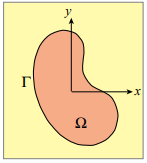
\includegraphics[width=0.2\textwidth]{Graphics/plane_stress.png}
    \caption{Plane stress problem}
    \label{fig:plane_stress}
\end{figure}

As we can see in the figure \ref{fig:plane_stress}, we have a the domain geometry $\Gamma$ and Specifified interior Forces, wich are known forces that act in the interior $\Omega$ of the plate.

Also one of the most important things are de Specified Surface Forces, these are known forces that act on the boundary $\Gamma$ and the displacement boundary conditions, these specify how the plate is supported.

\subsection{Problem Unkowns}

The unkown fields are the displacements, strains and stresses. 

\begin{align}
  \mathbf{u(x,y)} &=
  \begin{bmatrix}
      u_x(x,y) \\
      u_y(x,y)
  \end{bmatrix},
  &
  \mathbf{\epsilon(x,y)} &=
  \begin{bmatrix}
      e_{xx}(x,y) \\
      e_{yy}(x,y) \\
      2e_{xy}(x,y)
  \end{bmatrix}
  &
  \mathbf{\sigma(x,y)} &=
  \begin{bmatrix}
      \sigma_{xx}(x,y) \\
      \sigma_{yy}(x,y) \\
      \sigma_{xy}(x,y)
  \end{bmatrix}
\end{align}

\subsection{Governing equations}
The governing equations are the equilibrium equations, the strain-displacement equations and the stress-strain equations.
\begin{align}
    \epsilon= Du \\
    \sigma = E \epsilon \\
    D^T \sigma +b =0
\end{align}

Is important to note, that b is the body force vector, E is the 3x3 stress-strain matrix of plane stress elastic moduli D is th 3x2 symmetric-gradient operator and its s transpose the 2 × 3 tensor-divergence operator

\begin{align}
  \mathbf{D} &=
  \begin{bmatrix}
      \frac{\partial}{\partial x} & 0 \\
      0 & \frac{\partial}{\partial y} \\
      \frac{\partial}{\partial y} & \frac{\partial}{\partial x}
  \end{bmatrix}
  &
  \mathbf{E} &=
  \begin{bmatrix}
    E_{11} & E_{12} & E_{13} \\
    E_{21} & E_{22} & E_{23} \\
    E_{31} & E_{32} & E_{33}
  \end{bmatrix}
  &
  \mathbf{b} &=
  \begin{bmatrix}
      b_x \\
      b_y \\
  \end{bmatrix}
\end{align}

\subsection{boundary conditions}
There are two boundary conditions prescribed on $\Gamma$:
\begin{itemize}
    \item Discplacement boundary conditions ($\Gamma_u$): These are the displacements that are prescribed in the form of $u= \hat{u}$ .
    \item Force boundary conditions($\Gamma_t$): These are the forces that are prescribed in the form $\sigma_n= \hat{t}$.
\end{itemize}
To see it better, we can see the following figure:  
\begin{figure}[h]
    \centering
    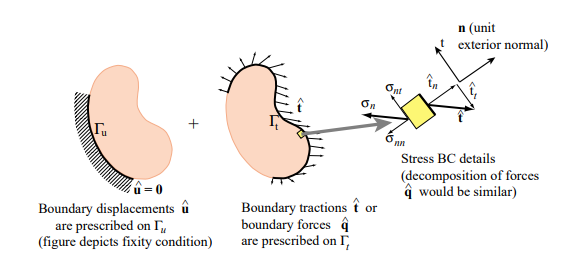
\includegraphics[width=0.7\textwidth]{Graphics/boundary_c1.PNG}
    \caption{Boundary conditions}
    \label{fig:boundary_conditions}
\end{figure}

\subsection{displacement interpolation}
The displacement field $u^e(x, y)$ over the element is interpolated from the node displacements. We
shall assume that the same interpolation functions are used for both displacement components
\begin{align}
  u_x(x,y)= \sum_{i=1}^{n} N_i^e(x,y) u_{xi}
  \hspace{1cm}
  u_y(x,y)= \sum_{i=1}^{n} N_i^e(x,y) u_{yi}
\end{align}

where $N_i^e (x, y)$ are the element shape functions. This N (with superscript e omitted to reduce clutter) is called the shape function matrix. It has dimensions 2 × 2n

\begin{align}
  \mathbf{N} &=
  \begin{bmatrix}
      N_1^e & 0     & N_2^e & 0 & \cdots &N_n^e & 0     \\
      0     & N_1^e & 0 & N_2^e & \cdots &0     & N_n^e
  \end{bmatrix}
\end{align}

Differentiating the finite element displacement field yields the strain-displacement relations:
\begin{align}
  \epsilon(x,y) &= D N \cdot u^e(x,y) = B \cdot u^e(x,y) 
\end{align}

This B = D N is called the strain-displacement matrix. It is dimensioned 3 × 2n

\begin{equation}
  \mathbf{B} =
  \begin{bmatrix}
      \frac{\partial N_1^e}{\partial x} & 0     & \frac{\partial N_2^e}{\partial x} & 0 & \cdots &\frac{\partial N_n^e}{\partial x} & 0     \\
      0     & \frac{\partial N_1^e}{\partial y} & 0 & \frac{\partial N_2^e}{\partial y} & \cdots &0     & \frac{\partial N_n^e}{\partial y} \\
      \frac{\partial N_1^e}{\partial y} & \frac{\partial N_1^e}{\partial x} & \frac{\partial N_2^e}{\partial y} & \frac{\partial N_2^e}{\partial x} & \cdots &\frac{\partial N_n^e}{\partial y} & \frac{\partial N_n^e}{\partial x}
  \end{bmatrix}
\end{equation}

\subsection{Element Stiffness Equations}
With the following relations, we can calculate the element stiffness matrix and the element force vector.
\begin{align}
  u = N u^e\\
  \epsilon = B u^e\\
  \sigma = E \epsilon
\end{align}

The element stiffness matrix is given by the following equation:

\begin{align}
  \mathbf{K}^e &= \int_{\Omega^e} h B^T E B d\Omega^e \\
\end{align}

and the consistent element nodal force vector is:
\begin{align}
  \mathbf{f}^e &= \int_{\Omega^e} h N^T b d\Omega^e +  \int_{\Gamma^e} h N^T \hat{t} d\Gamma^e\\
\end{align}

where $h$ is the thickness of the element, $b$ is the body force vector and $\Omega^e$ is the volume of the element.

Finally, we can describe the element stiffness matrix and the element force vector in a more compact form:

\begin{align}
  \int_{\Omega^e} h B^T E B d\Omega^e \cdot u = \int_{\Omega^e} h N^T b d\Omega^e +  \int_{\Gamma^e} h N^T \hat{t} d\Gamma^e \hspace{0.5cm} \rightarrow \hspace{0.5cm} \mathbf{K}^e \cdot u = \mathbf{f}^e
\end{align}

\subsection{}


\end{document} % Fin del documento